\documentclass{beamer}
\usetheme{Warsaw}
\usepackage{nhtvslides}
\usepackage{graphicx}
\usepackage{listings}
\usepackage{mathpartir}
\lstset{language=CAML,
basicstyle=\ttfamily\tiny,
frame=shadowbox,
breaklines=true,
mathescape=true}
\usepackage[utf8]{inputenc}


\title{Casanova: a language for game development}

\author{Candidate: G. Maggiore \inst{1,2} \and \\ Supervisors: M. Bugliesi \inst{1} \and P. Spronck \inst{3}}

\institute{\inst{1} Università Ca' Foscari - Venezia, Italy \and \inst{2} NHTV University - Breda, Netherlands \and \inst{3} Tilburg University, Netherlands}

\date{}

\AtBeginSection[]
{
    \begin{frame}{Outline}
        \tableofcontents[currentsection,currentsubsection]
    \end{frame}
}

\begin{document}
\maketitle

\begin{frame}{Table of contents}
\tableofcontents
\end{frame}

\section{Motivation}
\begin{slide}{Motivation}{Game development}{
\item Very large industry
\item Impact on 
\begin{itemize}
\item technology
\item culture
\item society
\end{itemize}
}\end{slide}

\begin{slide}{Motivation}{Challenges in game development}{
\item \textbf{Costs and complexity}...
\pause
\item ...resulting in less innovation
\item Especially by \textbf{smaller developers}
\begin{itemize}
\item independent (indie)
\item research
\item serious
\end{itemize}
}\end{slide}

\section{Making a game}
\begin{slide}{Making a game}{Structure of a game}{
\item \textbf{game world/state}
\item \textbf{game loop}
\begin{itemize}
\item continuous logic of the game world (\texttt{P := P + V * dt})
\item drawing of all drawables $\forall$ \texttt{d : Drawable} $\in$ \texttt{world do draw(d)}
\item discrete logic of the game world (\texttt{in\_room(player) -> light := ON})
\item \textbf{high performance}
\end{itemize}
}\end{slide}

\begin{frame}[fragile]{Structure of a game}
\begin{block}{Game world}
\begin{lstlisting}
class World {
  public List<Ship> Ships;
  public List<Planet> Planets;
  ...
}

class Ship {
  public Vector3 Position;
  public Vector3 Velocity;
  ...
  public Sprite HealthBar;
  public Model3D Appearance;
}

...
\end{lstlisting}
\end{block}
\end{frame}

\begin{frame}[fragile]{Structure of a game}
\begin{block}{Game loop}
\begin{lstlisting}
void Update(World world, float dt) {
  foreach(var s in world.Ships)
    if (!UpdateShip(world, s, dt))
      world.Ships.Remove(s);
  world.Ships.Add(NewShips(world, dt));
  ...
}
\end{lstlisting}
\end{block}
\end{frame}

\begin{frame}[fragile]{Structure of a game}
\begin{block}{Continuous dynamics}
\begin{lstlisting}
void UpdateShip(World w, Ship s, float dt) {
  s.Position += s.Velocity * dt;
  s.Velocity += s.Acceleration * dt;
  s.Life -= s.Damage(w) * dt;
  ...
  return s.Life > 0.0f;
}
\end{lstlisting}
\end{block}
\end{frame}

\begin{frame}[fragile]{Structure of a game}
\begin{block}{Drawing}
\begin{lstlisting}
void Draw(World world, float dt) {
  foreach(var s in world.Ships)
    DrawShip(s);
  ...
}

void DrawShip(s) {
  s.HealthBar.Transform = 
    Matrix.CreateTranslation(s.Position) *
    Matrix.CreateScale(s.Life, 1.0f, 1.0f);
  DrawSprite(s.HealthBar);
  s.Appearance.Transform = 
    Matrix.CreateTranslation(s.Position) *
    Matrix.CreateRotationY(atan2(norm(s.Velocity)));
  DrawModel3D(s.Appearance);
}
\end{lstlisting}
\end{block}
\end{frame}

\begin{frame}[fragile]{Structure of a game}
\begin{block}{Discrete dynamics (state machines)}
\begin{lstlisting}
class ShipSpawnTimer {
  public float Time;
  public bool Tick(float dt) {
    Time -= dt;
    if (Time <= 0.0f) {
      Time = ShipSpawnTime;
      return true;
    } else
      return false;
  }
}

Seq<Ship> NewShips(World world, float dt) {
  foreach(var s in world.ShipSpawnTimers)
    if(s.Tick(dt)) yield new Ship(...);
}
\end{lstlisting}
\end{block}
\end{frame}

\begin{frame}[fragile]{Structure of a game}
\begin{block}{Discrete dynamics (state machines)}
\begin{lstlisting}
class DragSelector {
  DragSelectionState state;
  Vector2 start;
  public Rectangle? Tick() {
    switch(state)
      case NotStarted:
        if (Mouse.LeftButton == ButtonState.Down) {
          state = Started;
          start = Mouse.Position;
          CreateSelectionRectangle(start);
          return null; }
      case Started:
        if (Mouse.LeftButton == ButtonState.Up) {
          state = Ended;
          end = Mouse.Position;
          return null; }
      case Ended:
        state = NotStarted;
        RemoveSelectionRectangle();
        return new Rectangle(start, end);
  }
}
\end{lstlisting}
\end{block}
\end{frame}

\begin{frame}[fragile]{Structure of a game}
\begin{block}{Optimization}
\begin{lstlisting}
class Ship {
  public float Damage(World w) {
    // use a spatial partitioning index to quickly find the 
    // adversary's ships close enough to this one to damage it
    ...
  }
\end{lstlisting}
\end{block}
\end{frame}

\begin{slide}{Game code}{The code above is:}{
\item \textbf{a lot:} traversing, updating, and drawing a large and complex game world
\item \textbf{error-prone:} explicit handling of state machines, keeping in sync update and draw code
\item \textbf{complex:} order of updates, order of draws, optimization algorithms
\item \textbf{boilerplate:} large portion of code not specific to the game
}\end{slide}

\begin{slide}{Game code}{Coping with complexity}{
\item \textbf{libraries} 
\begin{itemize}
\item low-level libraries of utilities
\item high-level OO libraries for game worlds (components)
\end{itemize}
\item \textbf{game engines}
\begin{itemize}
\item scripting for customizing an existing game
\item visual environment to fill the scene graph
\end{itemize}
}\end{slide}

\section{Casanova}
\begin{slide}{Casanova}{A game-development DSL}{
\item \textbf{part of the ML family}
\item \textbf{specific syntax and semantics}
\begin{itemize}
\item less code
\item less complexity
\item less boilerplate
\end{itemize}
\item \textbf{specific optimizations}
\begin{itemize}
\item higher performance
\item less complexity
\item less bugs
\end{itemize}
}\end{slide}

\begin{slide}{Casanova}{Features}{
\item \textbf{no game loop}
\item update logic through declarative, referentially transparent, local \textbf{rules}
\item \textbf{automated, declarative drawing} with transparent batching
\item state machines through (a calculus of) \textbf{coroutines}
\item \textbf{automated optimizations}
}\end{slide}

\begin{frame}[fragile]{Casanova}
\begin{block}{Syntax - ML Types}
\begin{lstlisting}
<type-decls> ::= <type-decl> | <type-decl> <type-decls>
<type-decl>  ::= `type' <id> `=' <type-body>
<type-body>  ::= <record-body> | <union-body>

<type-expr>   ::= <id> | <tuple-type-expr> | <intrinsic-type-expr>
<tuple-type-expr> ::= <type-expr> | <type-expr> `*' <tuple-type-expr>
<intrinsic-type-expr> ::= `Var<'<type-expr>`>' 
                        | `Ref<'<type-expr>`>' 
                        | `List<'<type-expr>`>' 
                        | `Coroutine<'<type-expr>`>' 
                        | float | int | Vector2 | ...
<union-body>  ::= <id> | <id> `of' <type-expr> 
                | <id> `|' <union-body> 
                | <id> `of' <type-expr> `|' <union-body>
\end{lstlisting}
\end{block}
\end{frame}
\begin{frame}[fragile]{Casanova}
\begin{block}{Syntax - Rules}
\begin{lstlisting}
<record-body> ::= `{' <labels> `}' <rules>
<labels>      ::= <label> | <label>`;' <labels>
<label>       ::= <id> `:' <type-expr>
<rules>       ::= empty | <rule> <rules>
<rule>        ::= `rule' <rule-id> `=' <expr>
<rule-id>     ::= <id> | <id>`.'<rule-id>
\end{lstlisting}
\end{block}
\end{frame}
\begin{frame}[fragile]{Casanova}
\begin{block}{Syntax - ML expressions}
\begin{lstlisting}
<type-init>    ::= <tuple-init> | <list-init> 
               | <record-init> | <union-init> | <intrinsic-type-init>
<tuple-init>   ::= <expr> | <expr>, <tuple-init>
<list-init>    ::= `[' <expr-list> `]' | `[' <list-compr> `]'
<list-compr>   ::= `for' <id> `in' <expr> `do' <expr>
<expr-list>    ::= `' | <expr> `;' <expr-list>
<record-init>  ::= `{' <labels-init> `}'
<labels-init>  ::= <id> `=' <expr> | <id> `=' <expr> `;' <labels-init>
<union-init>   ::= <id> | <id> <tuple-init>
<intrinsic-type-init> ::= `ref' <expr> | `var' <expr> 
               | `Vector2(' <expr> `,' <expr> `)' | ...
<type-dest>    ::= `let' <ids> `=' <expr> | <match-case> 
                 | `[]' | <id> `::' <id> | <id> `.' <id>
<match-case>   ::= `match' <expr> `with' <patterns>
<patterns>     ::= <pattern> | <pattern> `|' <patterns>
<pattern>      ::= <id> | <ids> | <id> `(' <pattern-args> `)'
<pattern-args> ::= <pattern-arg> | <pattern-arg> `,' <pattern-args>
<pattern-arg>  ::= <id> | <const>
<id-decl> ::= <id> | <id> `:' <type-expr>
<ids>          ::= <id> | <id> `,' <ids>
<id>      ::= ... (* an alphanumeric string *)
<const>   ::= ... (* a constant value *)
\end{lstlisting}
\end{block}
\end{frame}
\begin{frame}[fragile]{Casanova}
\begin{block}{Syntax - ML expressions/coroutines}
\begin{lstlisting}
<expr>    ::= <id> | <const> 
            | `let' <id> `=' <expr> `in' <expr> 
            | `if' <expr> `then' <expr> `else' <expr> 
            | <type-init> | <type-dest> 
            | <co-expr> | ...
<co-expr> ::= `co{' <co-expr> `}' | <expr> | `return' <expr> 
            | `let!' <id> `=' <expr> `in' <expr> 
            | `do!' <expr> `;' <expr> 
            | <expr> `||' <expr> | <expr> `&&' <expr> 
            | <expr> `=>' <expr> | `repeat' <expr> 
            | `yield'
\end{lstlisting}
\end{block}
\end{frame}
\begin{frame}[fragile]{Casanova}
\begin{block}{Syntax - Program}
\begin{lstlisting}
<p>             ::= <type-decls> <initial-world> <scripts>
<initial-world> ::= `let world =' <expr>
<scripts>       ::= <main-script> <input-script> 
<main-script>   ::= `let main =' <expr>
<input-script>  ::= `let input =' <expr>
\end{lstlisting}
\end{block}
\end{frame}
\begin{frame}[fragile]{Casanova}
\begin{block}{Typing rules}
\begin{lstlisting}
type E = { l1:T1; l2:T2; ... ln:Tn } 
  rule li = (ei:World * E * float<s> -> Ti)
\end{lstlisting}
\end{block}
\end{frame}
\begin{frame}[fragile]{Casanova}
\begin{block}{Typing rules}
\begin{lstlisting}
type E = { l1:T1; ...; li:{k1:V1; k2:V2; ... km:Vm} ln:Tn } 
  rule li.kj = (eij:World * E * float<s> -> Vj)
\end{lstlisting}
\end{block}
\end{frame}
\begin{frame}[fragile]{Casanova}
\begin{block}{ML-style typing rules}
\fontsize{6}{7.2}\selectfont
\begin{mathpar}
\inferrule
{\Gamma \vdash t_1:\texttt{U,}\ \Gamma,x:\texttt{U} \vdash t_2:\texttt{V}}
{\Gamma \vdash \texttt{let }x \texttt{=} t_1 \texttt{ in } t_2:V}

\inferrule
{\Gamma \vdash cond:\texttt{bool}, t_1:\texttt{U}, t_2:\texttt{U}}
{\Gamma \vdash \texttt{if }cond\texttt{ then }t_1\texttt{ else } t_2:U}

\inferrule
{\Gamma \vdash f:U \rightarrow V, t:U}
{\Gamma \vdash f t:V}

\inferrule
{\Gamma \vdash t:\{l_1:T_1;l_2:T_2;...l_n:T_n\}}
{\Gamma \vdash t.l_i:T_i}

...
\end{mathpar}
\end{block}
\end{frame}
\begin{frame}[fragile]{Casanova}
\begin{block}{Coroutines typing rules}
\fontsize{6}{7.2}\selectfont
\begin{mathpar}
\inferrule
{\Gamma \vdash t_1:\texttt{Var<T>}}
{\Gamma \vdash !t_1:\texttt{T}}

\inferrule
{\Gamma \vdash t_1:\texttt{Var<T>},t_2:\texttt{T}}
{\Gamma \vdash t_1:=t_2:\texttt{Co<Unit>}}

\inferrule
{\Gamma \vdash x:\texttt{T}}
{\Gamma \vdash \texttt{return } x:\texttt{Co<T>}}

\inferrule
{\Gamma \vdash t1:\texttt{Co<U>} \Gamma,x:\texttt{U} \vdash t2:\texttt{Co<V>}}
{\Gamma \vdash \texttt{let! } x \texttt{=} t1 \texttt{ in } t2:\texttt{Co<V>}}

\inferrule
{}
{\vdash \texttt{yield}:\texttt{Co<Unit>}}

\inferrule
{\Gamma \vdash t:\texttt{float<s>}}
{\Gamma \vdash \texttt{wait }t:\texttt{Co<Unit>}}

\inferrule
{\Gamma \vdash t_1:\texttt{Co<U>},t_2:\texttt{Co<V>}}
{\Gamma \vdash t_1\texttt{ \&\& }t_2:\texttt{Co<U*V>}}

\inferrule
{\Gamma \vdash t_1:\texttt{Co<U>},t_2:\texttt{Co<V>}}
{\Gamma \vdash t_1 \texttt{ || } t_2:\texttt{Co<Either<U,V>>}}

\inferrule
{\Gamma \vdash t_1:\texttt{Co<bool>},t_2:\texttt{Co<V>}}
{\Gamma \vdash t_1 \texttt{ => } t_2:\texttt{Co<V>}}

\inferrule
{\Gamma \vdash t:\texttt{Co<Unit>}}
{\Gamma \vdash \texttt{repeat }t:\texttt{Co<Unit>}}
\end{mathpar}
\end{block}  
\end{frame}

\begin{frame}[fragile]{Casanova}
\begin{block}{Overall game semantics}
\begin{lstlisting}
let rec update world dt =
  let world'  = apply_rules world dt
  let world'' = tick_scripts world'
  do draw world''
  update world'' dt
\end{lstlisting}
\end{block}
\end{frame}
\begin{frame}[fragile]{Casanova}
\begin{block}{World traversal semantics}
\begin{lstlisting}
apply_rules (world:World) (dt:float<s>) = update_world [World] world dt

update_world [World] (world:World) (dt:float<s>) = 
  update_entity [World] [World] world world dt

update_entity [World] [Primitive(T)] 
              (world:World) (v:T) dt = ()
update_entity [World] [T1 * T2 * ... * Tn] 
              (world:World) (x1:T1, x2:T2, ..., xn:Tn) dt =
  update_entity [World] [T1] world x1 dt 
  update_entity [World] [T2] world x2 dt
  ...
  update_entity [World] [Tn] world xn dt
update_entity [World] [Var<T>] 
              (world:World) (v:Var<T>) dt = 
  update_entity [World] [T] (world:World) !v dt
update_entity [World] [Ref<T>] 
              (world:World) (v:Ref<T>) dt = ()
update_entity [World] [List<T>] 
              (world:World) (l:List<T>) dt =
  for x in l do update_entity [World] [T] world x dt
\end{lstlisting}
\end{block}
\end{frame}
\begin{frame}[fragile]{Casanova}
\begin{block}{World traversal semantics}
\begin{lstlisting}
update_entity [World] [T=UnionCase(C1(T11 * ... * T1n1), 
                                   C2(T21 * ... * T2n2), ..., 
                                   Cn(Tn1 * ... * Tnnn)))] 
              (world:World) (c:T) dt =
  match c with
  | C1(x1,...,xn1) ->
    update_entity [World] [T11] world x1 dt
    update_entity [World] [T12] world x2 dt
    ...
    update_entity [World] [T1n1] world xn1 dt
  | C2(x1,...,xn2) ->
    update_entity [World] [T21] world x1 dt
    update_entity [World] [T22] world x2 dt
    ...
    update_entity [World] [T2n1] world xn2 dt
  ...
  | Cn(x1,...,xnn) ->
    update_entity [World] [Tn1] world x1 dt
    update_entity [World] [Tn2] world x2 dt
    ...
    update_entity [World] [Tnnn] world xnn dt
\end{lstlisting}
\end{block}
\end{frame}
\begin{frame}[fragile]{Casanova}
\begin{block}{Rule application semantics}
\begin{lstlisting}
update_entity [World] [T=Record(l1:T1,l2:T2,...,ln:Tn,
                                r1=rb1,r2=rb2,...,rm=rbm)] 
              (world:World) (r:T) dt =
  update_entity [World] [T1] world r.l1 dt
  update_entity [World] [T2] world r.l2 dt
  ...
  update_entity [World] [Tn] world r.ln dt
  r.r1 := rb1(world, r, dt)
  r.r2 := rb2(world, r, dt)
  ...
  r.rm := rbm(world, r, dt)
\end{lstlisting}
\end{block}
\end{frame}
\begin{frame}[fragile]{Casanova}
\begin{block}{Coroutines semantics}
\begin{lstlisting}
type ScriptStep<s,a> = Done of a * s | Next of Script<s,a> * s
and Script<s,a> = s $\rightarrow$ ScriptStep<s,a>

let s1 >>= s2 =
  fun s ->
    match s1 s with
    | Done(x,s') -> Next(s2 x,s')
    | Next(k,s') -> Next(k >>= s2,s')

let return x = fun s -> Done x

let yield = fun s -> Right(s, (fun s -> ((),s)))
\end{lstlisting}
\end{block}
\end{frame}
\begin{frame}[fragile]{Casanova}
\begin{block}{Coroutines operators semantics}
\begin{lstlisting}
let (&&) (p:Co<'a>) (q:Co<'b>) : Co<'a * 'b> =
  match p(), q() with
  | Done x, Done y -> Done(x,y)
  | Next p', Next q' -> Next (p' && q')
  | Next p', Done y -> Next(p' && return y)
  | Done x, Next q' -> Next(return x && q')

let (||) (p:Co<'a>) (q:Co<'b>) : Co<Choice<'a,'b>> =
  match p(), q() with
  | Done x, _ -> Done(Choice1Of2 x)
  | _, Done y -> Done(Choice2Of2 y)
  | Next p', Next q' -> Next (p' || q')

let repeat (p:Co<Unit>) : Co<Unit> = p >>= (fun _ -> repeat p)
\end{lstlisting}
\end{block}
\end{frame}
\begin{frame}[fragile]{Casanova}
\begin{block}{Draw batching semantics}
\begin{lstlisting}
layers = []
draw_world [World] (world:World) = 
  draw_entity [World] world
  for layer in layers do
    layer.Draw()
    layer.Clear()
\end{lstlisting}
\end{block}
\end{frame}
\begin{frame}[fragile]{Casanova}
\begin{block}{Draw traversal semantics}
\begin{lstlisting}
draw_entity [Primitive(T)] (v:T) = ()
draw_entity [T1 * T2 * ... * Tn] (x1:T1, x2:T2, ..., xn:Tn) =
  draw_entity [T1] x1
  ...
  draw_entity [Tn] xn
draw_entity [Var<T>] (v:Var<T>) = draw_entity [T] !v
draw_entity [Ref<T>] (v:Ref<T>) = ()
draw_entity [List<T>] (l:List<T>) =
  for x in l do draw_entity [T] x
\end{lstlisting}
\end{block}
\end{frame}
\begin{frame}[fragile]{Casanova}
\begin{block}{Draw traversal semantics}
\begin{lstlisting}
draw_entity [T=UnionCase(C1(T11 * ... * T1n1), 
                         Cn(Tn1 * ... * Tnm)))] (c:T) =
  match dt with
  | C1(x1,...,xn1) ->
    draw_entity [T11] x1
    ...
    draw_entity [T1n1] xn1
  ...
  | Cn(x1,...,xnm) ->
    draw_entity [Tn1] x1
    ...
    draw_entity [Tnm] xnm

draw_entity [T=Record(l1:T1,l2:T2,...,ln:Tn,rules)] (r:T) =
  draw_entity [T1] r.l1
  ...
  draw_entity [Tn] r.ln
\end{lstlisting}
\end{block}
\end{frame}
\begin{frame}[fragile]{Casanova}
\begin{block}{Actual drawing semantics}
\begin{lstlisting}
draw_entity [Drawable(T)] (d:T) = d.Layer.AddT(d)
draw_entity [Layer(T)] (l:T) = layers.Add(l)
\end{lstlisting}

\footnotesize{Note: easily extensible with additional drawable datatypes.}
\end{block}
\end{frame}

\begin{frame}[fragile]{Structure of a game}
\begin{block}{Game of life}
\begin{lstlisting}
type World = { 
  Cells : List<Cell> 
  UpdateNow : Var<bool> 
}

type Cell = { 
  Position : Vector2<m>
  Value    : int 
  Sprite   : Sprite }
  rule Value(world,self,dt) = 
    if world.UpdateNow then 
      let around = sum [for c in world.Cells do 
                          if dist(self.Position, c.Position < 1.5f<m> then 
                            yield c.Value] 
      match around with 
      | 3 -> 1 
      | 2 -> self.Value 
      | _ -> 0 
    else self.Value 
  rule Sprite.Color(world,self,dt) = 
    if self.Value = 0 then Color.Black else Color.White
\end{lstlisting}
\end{block}
\end{frame}
\begin{frame}[fragile]{Casanova}
\begin{block}{Structure of a game}
\begin{lstlisting}
let main world = 
  repeat co{ 
    do! wait 1.0<s> 
    do! world.UpdateNow := true 
    do! yield 
    do! world.UpdateNow := false } 

let input = [
    wait_key_down Keys.Space =>
     co{
       do! world.UpdateNow := true
       do! yield
       do! world.UpdateNow := false }
  ]
\end{lstlisting}
\end{block}
\end{frame}

\begin{slide}{Casanova}{Implementation}{
\item presented syntax is not implemented in practice
\item \textit{embedding} into F\#, leveraging existing high quality:
\begin{itemize}
\item development environment
\item debugging tools
\item libraries (MonoGame)
\end{itemize}
\item Casanova compiler
\begin{itemize}
\item compiles a \textit{stub} dll with the F\# compiler
\item \textit{reflects} the existing type and script definitions
\item \textit{emits} the missing functionality in the final dll
\end{itemize}
}\end{slide}

\begin{frame}[fragile]{Casanova}
\begin{block}{Type translation into F\#}
\begin{lstlisting}
translate_types [] = ()
translate_types type::types = 
  translate_type type
  translate_types types

translate_type Primitive(type) = type
translate_type Var<type> = Var<translate_type type>
translate_type List<type> = List<translate_type type>
translate_type Union(cases) = Union([translate_case case | case in cases])
translate_type Tuple(types) = Tuple([translate_type type | type in types])
translate_type Record(labels,rules) = Record([translate_label label rules | label in labels])

translate_case UnionCase(case,types) = UnionCase(case, [translate_type type | type in types])
translate_label Label(name,type) rules = 
  if exists(rule.Name = name) in rules then
    if type = List<type'> then
      Label(name,RuleList<translate_type type'>)
    else
      Label(name,Rule<translate_type type'>)
\end{lstlisting}
\end{block}
\end{frame}
\begin{frame}[fragile]{Casanova}
\begin{block}{Rule double buffering}
\begin{lstlisting}
type Rule<'T> = { 
  mutable current : 'T; 
  mutable next : 'T }

let (!) r = r.current
let (:=) r v' = r.next <- v'
\end{lstlisting}
\end{block}
\end{frame}

\begin{slide}{Casanova}{Optimizations}{
\item aggressive inlining
\item multi-threaded draw/update
\item memory recycling across frames
\item batched drawing
}\end{slide}

\section{Evaluation}
\begin{tableslide}{Evaluation}{Comparison with other languages}{| p{3cm} | c | c | c | c |}{
\hline
 & Cnv & C\#/XNA & pygame & C++/DX \\
\hline
Game loop & V & V & V & V \\
State traversal & V & X & X & X \\
State machines & V & X (iter.) & X (iter.) & X \\
Drawing & V & X & V & X \\
High performance & V & V & X & V \\
\hline
}\end{tableslide}

\begin{frame}[fragile]{Structure of a game}
\begin{columns}
\column{5cm}
\large{C\#}
\begin{lstlisting}
class World {
  public List<Ship> Ships;
  public List<Planet> Planets;
  ...
}
\end{lstlisting}
\column{5cm}
\large{Casanova}
\begin{lstlisting}
type World = {
  Ships   : List<Ship>
  Planets : List<Planet>
  ...
}
\end{lstlisting}
\end{columns}
\end{frame}

\begin{frame}[fragile]{Structure of a game}
\begin{columns}
\column{5cm}
\large{C\#}
\begin{lstlisting}
void Update(World world, float dt) {
 foreach(var s in world.Ships)
   if (!UpdateShip(world, s, dt))
     world.Ships.Remove(s);
 world.Ships.Add(NewShips(world,dt));
  ...
}
\end{lstlisting}
\column{5cm}
\large{Casanova}
\begin{lstlisting}
type World = {
  ..
} rule Ships = 
   [for s in self.Ships do 
     if s.Life > 0.0f then yield s]
\end{lstlisting}
\footnotesize{One less source of bugs for free!}
\end{columns}
\end{frame}

\begin{frame}[fragile]{Structure of a game}
\begin{columns}
\column{5cm}
\large{C\#}
\begin{lstlisting}
void UpdateShip(World w, Ship s, float dt) {
  s.Position += s.Velocity * dt;
  s.Velocity += s.Acceleration * dt;
  s.Life -= s.Damage(w) * dt;
  ...
  return s.Life > 0.0f;
}
\end{lstlisting}
\column{5cm}
\large{Casanova}
\begin{lstlisting}
type Ship = {
  ...
 } rule Position  = self.Position + self.Velocity * dt
   rule Velocity  = self.Velocity + self.Acceleration * dt
   rule Life      = self.Life - ...
\end{lstlisting}
\end{columns}
\end{frame}

\begin{frame}[fragile]{Structure of a game}
\begin{columns}
\column{5cm}
\large{C\#}
\begin{lstlisting}
void Draw(World world, float dt) {
  foreach(var s in world.Ships)
    DrawShip(s);
  ...
}

void DrawShip(s) {
  s.HealthBar.Transform = 
    Matrix.CreateTranslation(s.Position) *
    Matrix.CreateScale(s.Life, 1.0f, 1.0f);
  DrawSprite(s.HealthBar);
  s.Appearance.Transform = 
    Matrix.CreateTranslation(s.Position) *
    Matrix.CreateRotationY(atan2(norm(s.Velocity)));
  DrawModel3D(s.Appearance);
}
\end{lstlisting}
\column{5cm}
\large{Casanova}
\begin{lstlisting}
type Ship = {
  ...
  HealthBar  : Line
  Appearance : Model
 } rule HealthBar.Position  = self.Position
   rule HealthBar.Length    = self.Life
   rule Appearance.Position = self.Position
   rule Appearance.Rotation = atan2(norm(s.Velocity))
\end{lstlisting}
\end{columns}
\end{frame}

\begin{frame}[fragile]{Structure of a game}
\begin{columns}
\column{5cm}
\large{C\#}
\begin{lstlisting}
class ShipSpawnTimer {
  public float Time;
  public bool Tick(float dt) {
    Time -= dt;
    if (Time <= 0.0f) {
      Time = ShipSpawnTime;
      return true;
    } else
      return false;
  }
}

Seq<Ship> NewShips(World world, float dt) {
  foreach(var s in world.ShipSpawnTimers)
    if(s.Tick(dt)) yield new Ship(...);
}
\end{lstlisting}
\column{5cm}
\large{Casanova}
\begin{lstlisting}
repeat
 co{
   do! wait ShipSpawnTime
   do! world.Ships.Add(new Ship(...))
 }
\end{lstlisting}
\end{columns}
\end{frame}

\begin{frame}[fragile]{Structure of a game}
\begin{columns}
\column{5cm}
\large{C\#}
\begin{lstlisting}
class DragSelector {
  DragSelectionState state;
  Vector2 start;
  public Rectangle? Tick() {
    switch(state)
      case NotStarted:
        if (Mouse.LeftButton == ButtonState.Down) {
          state = Started;
          start = Mouse.Position;
          CreateSelectionRectangle(start);
          return null; }
      case Started:
        if (Mouse.LeftButton == ButtonState.Up) {
          state = Ended;
          end = Mouse.Position;
          return null; }
      case Ended:
        state = NotStarted;
        RemoveSelectionRectangle();
        return new Rectangle(start, end); } }
\end{lstlisting}
\column{5cm}
\large{Casanova}
\begin{lstlisting}
repeat
 co{
   let! start = wait_left_mouse_down
   do CreateSelectionRectangle(start)
   let! end = wait_left_mouse_up
   do RemoveSelectionRectangle()
 }
\end{lstlisting}
\end{columns}
\end{frame}

\begin{tableslide}{Evaluation}{Comparisong with systems}{| p{3cm} | c | c | c |}{
\hline
 & Cnv & Unity & Game maker \\
Game loop & V & V & V \\
State traversal & V & V & V \\
State machines & V & V (no ser.) & X \\ 
Drawing & V & V & V \\ 
Comparison & V & V & X \\
Custom games & V & V (fixed comp.) & X \\
\hline
}\end{tableslide}

\begin{slide}{Evaluation}{Making games with Casanova?}{
\item several samples
\item research prototypes
\item student games
\item even a commercial game!
}\end{slide}

\begin{frame}[fragile]{Evaluation}
\textbf{DEMO}

\begin{columns}[c]
\column{1.5in}
\begin{figure}
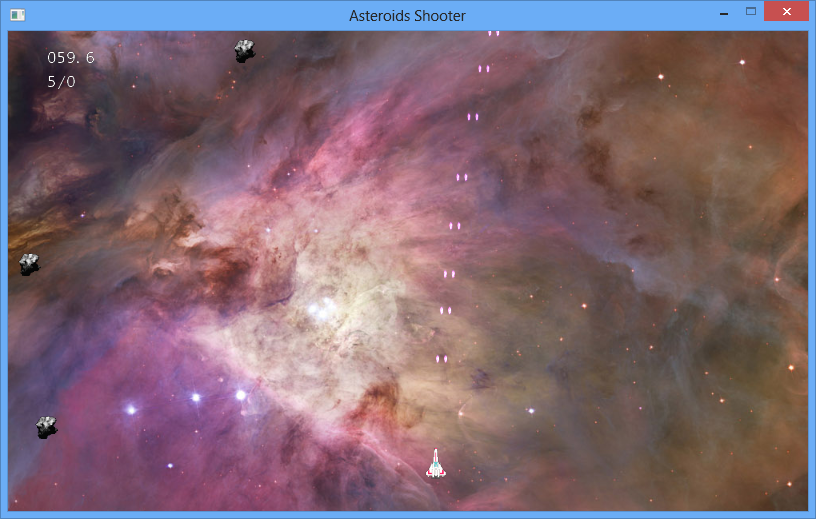
\includegraphics[scale=0.15]{Pics/asteroid_shooter.png}
\end{figure}
\begin{figure}
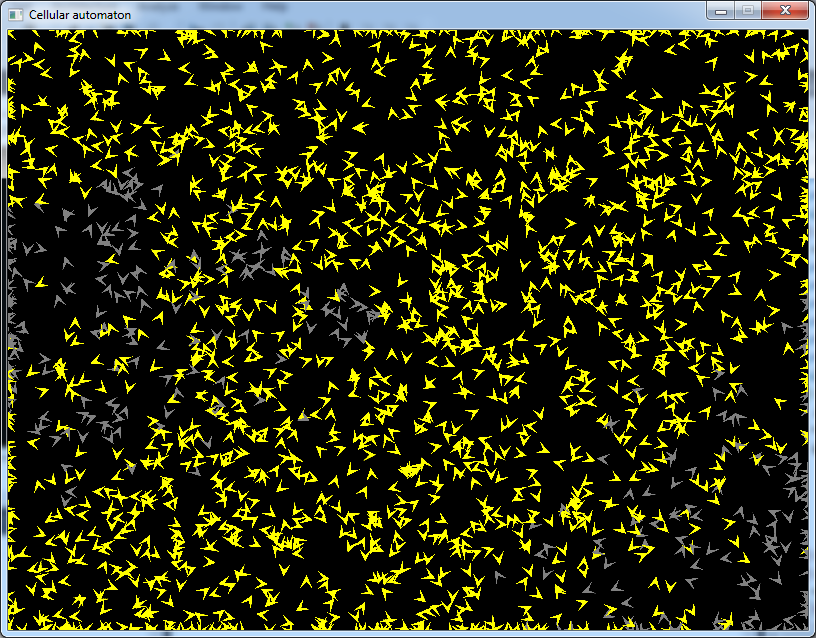
\includegraphics[scale=0.15]{Pics/cellular_automaton.png}
\end{figure}

\column{1.5in}
\begin{figure}
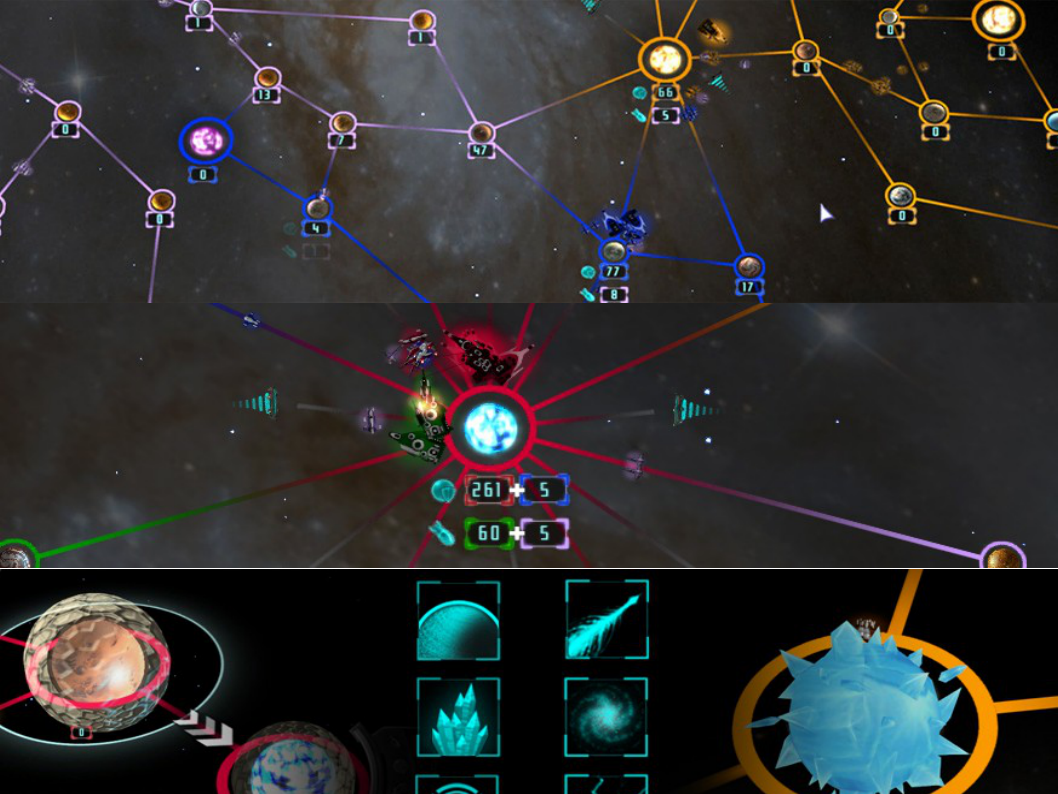
\includegraphics[scale=0.1]{Pics/galaxy_wars.png}
\end{figure}
\begin{figure}
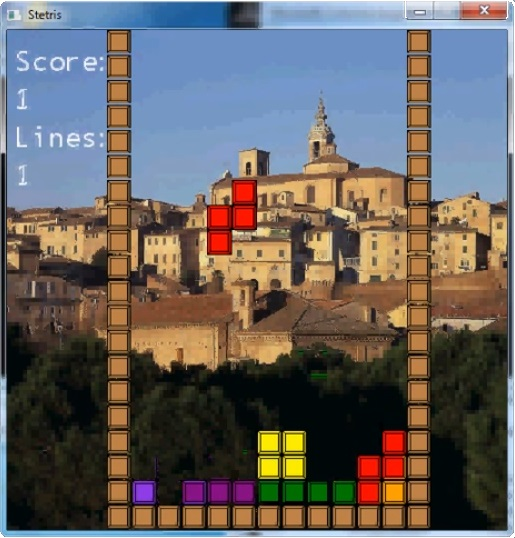
\includegraphics[scale=0.15]{Pics/tetris.jpg}
\end{figure}

\column{1.5in}
\begin{figure}
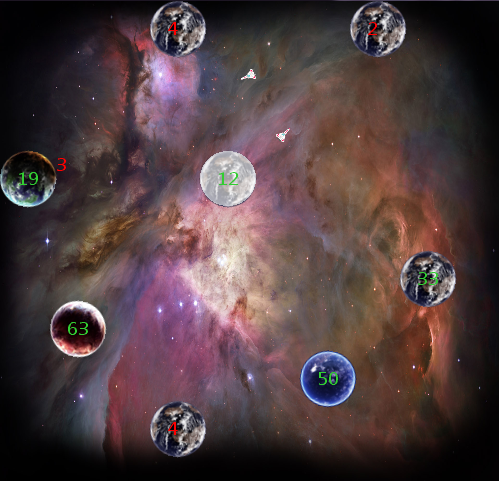
\includegraphics[scale=0.15]{Pics/RTS.png}
\end{figure}
\begin{figure}
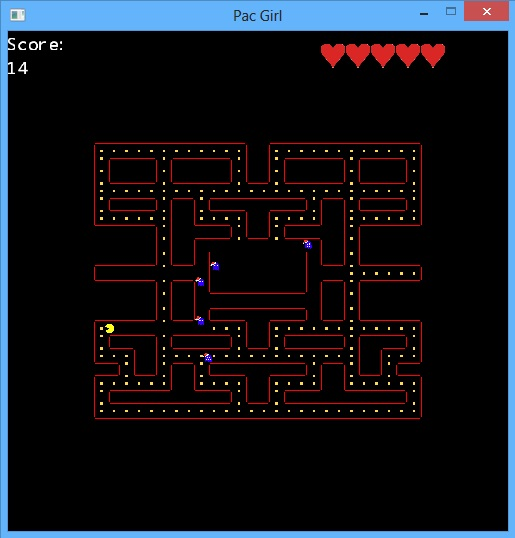
\includegraphics[scale=0.15]{Pics/pacman.jpg}
\end{figure}
\end{columns}
\end{frame}

\section{Future work \& conclusions}
\begin{slide}{Future work}{Already built}{
\item SQL-style, declarative actions to implement resource economies
\item declarative menus and global state transitions
\item nesting of visuals for relative positioning
\item actual assembly, no interpretation steps
}\end{slide}

\begin{frame}[fragile]{About actions}
\begin{columns}
\column{5cm}
\large{C\#}
\begin{lstlisting}
class Ship {
  public float Damage(World w) {
    // use a spatial partitioning index to quickly find the 
    // adversary's ships close enough to this one to damage it
    ...
  }
\end{lstlisting}
\column{5cm}
\large{Casanova}
\begin{lstlisting}
type Ship = {
  ...
  FightAction : TARGET Fleet
                RESTRICTION <>Owner and 
                RADIUS < 150.0f
                TRANSFER Life - 1.0
}
\end{lstlisting}
\end{columns}
\end{frame}

\begin{slide}{Future work}{Under construction}{
\item networking support
\item support for mobile/non-Windows platforms
\item support for 3D and hierarchical visibility culling
\item integration with Unity 3D
\item audio support
\item compiler front-end
\item static analysis tools and techniques (correct dynamics, load upper bounds)
}\end{slide}

\begin{slide}{Conclusions}{Impact of Casanova}{
\item game development is \textbf{relevant}
\item game development is \textbf{expensive}
\item Casanova makes it \textbf{easier, quicker, and safer}
\item hopefully to the benefit of smaller developers: \textbf{indie, research, and serious}
}\end{slide}

\begin{slide}{Conclusions}{Relevant publications - preliminary studies}{
\fontsize{6}{10}\selectfont
\item Giuseppe Maggiore, Michele Bugliesi, and Renzo Orsini. Monadic scripting in F\# for computer games. \textit{TTSS, 2011}.
\item Giuseppe Maggiore, Fabio Pittarello, Michele Bugliesi, and Mohamed Abbadi. A compilation technique to increase x3d performance and safety. \textit{SAC, 2012}.
\item G. Maggiore and G. Costantini. Friendly F\# (\textit{book}).
}\end{slide}

\begin{slide}{Conclusions}{Relevant publications - Casanova}{
\fontsize{6}{10}\selectfont
\item Giuseppe Maggiore, Alvise Spanò, Renzo Orsini, Giulia Costantini, Michele Bugliesi, and Mohamed Abbadi. Designing casanova: A language for games. \textit{ACG, 2011}.
\item Giuseppe Maggiore, Alvise Spanò, Renzo Orsini, Michele Bugliesi, Mohamed Abbadi, and Enrico Steffinlongo. A formal specification for casanova, a language for computer games. \textit{EICS, 2012}.
\item Giuseppe Maggiore, Renzo Orsini, and Michele Bugliesi. On casanova and databases or the similarity between games and dbs. \textit{SEBD, 2012}.
\item Giuseppe Maggiore, Pieter Spronck, Renzo Orsini, Michele Bugliesi, Enrico Steffinlongo, and Mohamed Abbadi. Writing real-time .Net games in casanova. \textit{ICEC, 2012}.
}\end{slide}

\begin{slide}{Conclusions}{Relevant publications - work in progress}{
\fontsize{6}{10}\selectfont
\item LGOAP: adaptive layered planning for real-time videogames. Giuseppe Maggiore, Carlos Santos, Dino Dini, Frank Peters, Hans Bouwknegt, and Pieter Spronck (\textit{submitted to IEEE 2013 Conference on Computational Intelligence in Games}).
\item The Domain of Parametric Hypercubes for Static Analysis of Computer Games Software. Giulia Costantini, Pietro Ferrara, Giuseppe Maggiore, and Agostino Cortesi (\textit{submitted to 15th International Conference on Formal Engineering Methods}).
\item Resources, Entities, Actions. A generalized design pattern for RTS games and its
  language extension in Casanova. Mohamed Abbadi, Francesco Di Giacomo, Renzo Orsini, Aske Plaat, Pieter Spronck, and Giuseppe Maggiore. (\textit{submitted to 8TH INTERNATIONAL CONFERENCE ON COMPUTER AND GAMES 2013}).
}\end{slide}

\begin{slide}{Conclusions}{Relevant publications - our game}{
\fontsize{6}{10}\selectfont
\item Galaxy Wars. \url{http://www.galaxywarsthegame.com/}.
}\end{slide}

\begin{frame}{This is it}
\begin{block}{Thank you!}
Questions?
\end{block}
\end{frame}

\end{document}
